\documentclass[conference]{IEEEtran}
%\documentclass[letterpaper,10pt]{article}

\usepackage[utf8]{inputenc}
\usepackage{kpfonts}
\usepackage[top=1in, bottom=1in, left=1in, right=1in]{geometry}
\usepackage{parskip}
\usepackage{tabularx}
\usepackage{qtree}
\usepackage{graphicx}
\usepackage{xfrac}
\usepackage{forest}
\usepackage{tikz-dependency}
\usepackage{graphicx}
\usepackage{float}
\usepackage{amsmath}
\usepackage{varioref}
\usepackage{hyperref}
\usepackage{xfrac}
\usepackage{amsmath}
\usepackage{bm}
\usepackage{pgfplots}
\usepackage{pbox}
\usepackage{framed}
\usepackage[authordate,bibencoding=auto,strict,backend=biber,natbib]{biblatex-chicago}
\usepackage{comment}
\usepackage{enumitem}
\usepackage{float}
\usepackage{dblfloatfix}
\usepackage{afterpage}
\usepackage{multirow}
%\usepackage[section]{placeins}


\renewcommand{\cite}{\citep}
\numberwithin{equation}{section}
\renewcommand{\tabularxcolumn}[1]{>{\small}m{#1}}

\def\topfraction{0.9} % 90 percent of the page may be used by floats on top
\def\bottomfraction{0.9} % the same at the bottom
\def\textfraction{0.01}


%\pdfinfo{
%   /Author (Gaurav Manek)
%   /Title  (Incrementally Identifying Objects from Referring Expressions using Spatial Object Models)
%   /CreationDate (D:20160210120000)
%   /Subject (Incremental Parsing)
%   /Keywords (Incremental;Parsing;Referring Expressions;Prepositions)
%}

%\newcommand{\sectionbreak}{\clearpage}

\DeclareMathOperator*{\argmin}{arg\,min}
\DeclareMathOperator*{\argmax}{arg\,max}

% http://tex.stackexchange.com/a/33547
\newcommand{\approptoinn}[2]{\mathrel{\vcenter{
  \offinterlineskip\halign{\hfil$##$\cr
    #1\propto\cr\noalign{\kern2pt}#1\sim\cr\noalign{\kern-2pt}}}}}

\newcommand{\appropto}{\mathpalette\approptoinn\relax}

\addbibresource{prop.bib}

%opening
\title{Incrementally Identifying Objects from Referring Expressions using Spatial Object Models}
\author{Gaurav Manek\\(Advisor: Prof. Stefanie Tellex)}

\begin{document}

\maketitle


\section{Introduction}

Referring expressions are phrases used to identify a particular object in a scene by describing it and its relative position to other objects. The integration of \emph{social feedback}, where the robot shows its understanding of a human's utterances by generating small responses as it listens to the human, can prompt clarifications from the human and improve the accuracy of referring expression parsing in interactive contexts. However, this requires robots to be able to parse the human input \emph{incrementally}: updating its understanding as each next word is uttered. 

In this paper we present an incremental referring expression parser that can process prepositional phrases. The incremental nature of the parser is the key contribution: state-of-the-art parsers all operate on complete referring expressions. 

In current work, referring expression parsing is done in batch-mode, with the entire referring expression as input. \citep{tellex2011understanding,UW_RSE_ICML2012,artzi2013weakly,fang2015embodied} During interactive use, batch-mode requires waiting for the complete utterance before processing and providing output, which introduces unaccceptable latency in the robot's response. For example, practical implementations of the $G^3$ system, as created by \citet{tellex2011understanding}, can take up to 30 seconds from the end of the input to the start of a response. Our incremental parsing system updates the distribution with each added word, substantially reducing the delay between input and response.

The incremental parser works by using a conditional-random field chunker to add parts of speech tags to sentences. These tags are used to construct a parse tree, which is then evaluated using an object-word model to resolve references to objects and a preposition model to resolve prepositional phrases. A caching method avoids recomputation cost and gives good worst-case time guarantees.

We evaluate our model on novel real-world data and show that it assigns the correct object the highest probability 32.8\% of the time and in the top-3 objects 63.5\% of the time. In comparison, humans correctly identify the object 79.0\% of the time, a unigram model 16.1\% of the time and random selection is only correct 7.2\% of the time. We also show how incremental performance converges to the above values as more words are available.

\begin{figure}[!tb]
  \centering
    \fbox{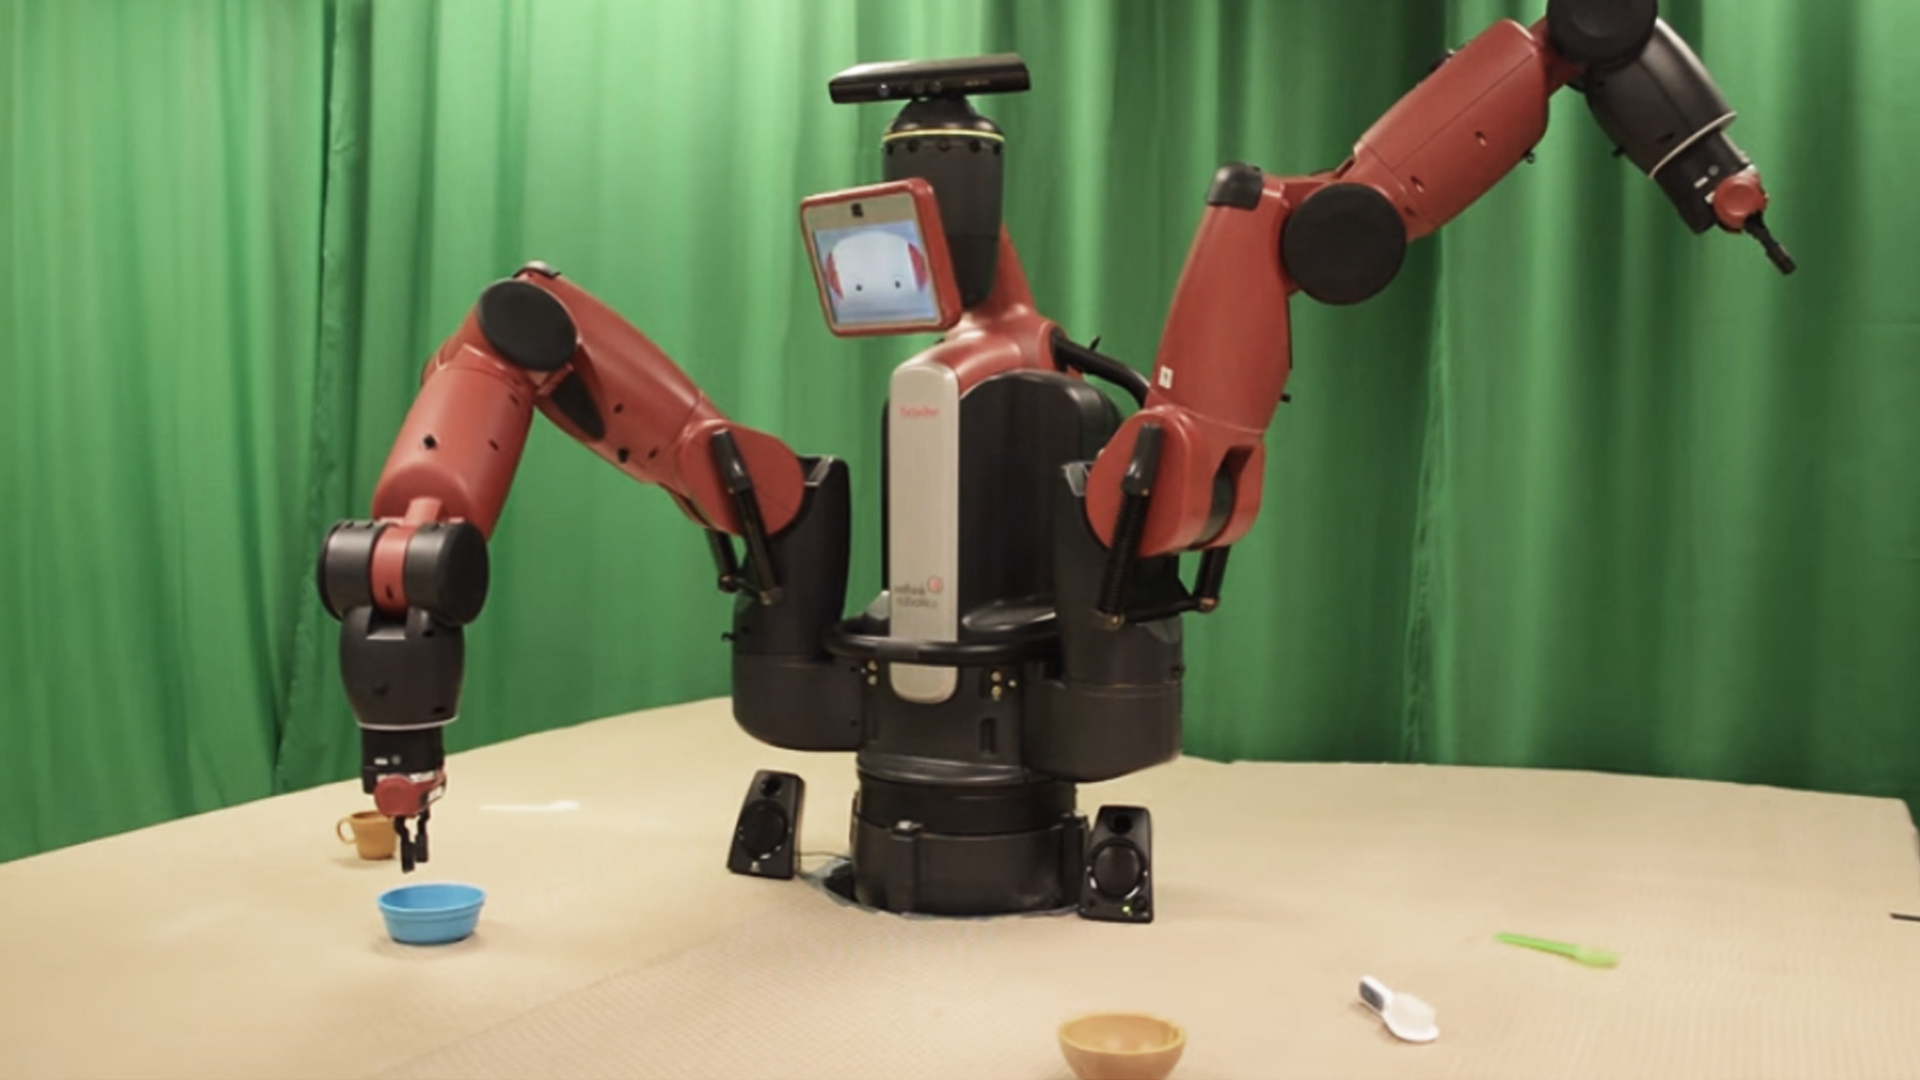
\includegraphics[width=0.9\columnwidth]{baxter}}
  \label{fig:robot}

  \caption{Baxter Robot in H2R lab, Brown University.}
\end{figure}

Figure~\ref{fig:worked_example} shows an example of the incremental parsing of a referring expression. As more words are available to the parser, the parser identifies the target object by assigning it the highest probability.



\section{Technical Approach}

\afterpage{%
\begin{figure*}[tb]
\begin{tabularx}{\textwidth}{@{} >{\hsize=.5\hsize \centering}X >{\hsize=.45\hsize}X @{}} 
\multicolumn{2}{c}{``The orange cube between the red thing and the yellow thing.''} \\ 
\multicolumn{2}{c}{$\Downarrow$} \\ 
% Chunking	
\begin{tabular}{c}
$\underbrace{\text{The orange cube}}_{\texttt{SNP}}$
$\underbrace{\text{between}}_{\texttt{PRP}}$
$\underbrace{\text{the red thing}}_{\texttt{SNP}}$
\\
$\underbrace{\text{and}}_{\texttt{PRP}}$
$\underbrace{\text{the yellow thing}}_{\texttt{SNP}}$
$\underbrace{\text{.}}_{\texttt{.}}$
\end{tabular}
& 
\textbf{Chunking}

First, we use Mallet, \citep{McCallumMALLET} a sequence tagging library, to tag the referring expression with a set of tags. The tags were developed to suit our use case, and are a simplification of the typical English parts-of-speech tags.

\\ $\Downarrow$ \\[0.2cm] 

\scalebox{.9}{\Tree [.TARGET \qroof{The orange cube}.OBJECT [.BETWEEN   \qroof{the red thing}.OBJECT \qroof{the yellow thing}.OBJECT ] ]} &

\textbf{Semantic Tree}

The tagged sequence is then converted to a semantic tree. Because of the simplified tag set in the previous step, this transformation is deterministic.

\\ $\Downarrow$ \\[0.2cm] 

\scalebox{.9}{\Tree [.TARGET \qroof{$\{\sfrac{1}{16}, \sfrac{1}{16}, \ldots, \sfrac{1}{16}\}$}.OBJECT [.BETWEEN   \qroof{$\{0, \sfrac{1}{8}, \ldots, 0\}$}.OBJECT \qroof{$\{0, 0, \ldots, \sfrac{1}{2}\}$}.OBJECT ] ]} 

~

\scriptsize{\{\textit{orange\_1}, \textit{red\_1}, $\ldots $, \textit{yellow\_2}\}}

&
\textbf{Language Model}

We use a language model to convert each of the simple noun phrases into individual distributions over possible objects.

\\ $\Downarrow$ & ~ \\[0.2cm] 

\scalebox{.9}{\Tree [.TARGET \qroof{$\{90\%, 2\%, \ldots 1\%\}$}.OBJECT ]} 

~

\scriptsize{\{\textit{orange\_1}, \textit{orange\_2}, $\ldots $, \textit{blue\_1}\} }

&
\textbf{Bottom-up Evaluation}

We evaluate the tree from the bottom upwards, using spatial features and trained weights to convert each input distribution and the type of preposition into a set of output scores. The final result is the object with the highest score.
\end{tabularx}
\caption{The processing steps in our algorithm.}
\label{fig:proc_flow}
\end{figure*}
\clearpage

\begin{figure*}[tb]
\newcommand{\inctest}[1]{\includegraphics[trim={0 3cm 5cm 3.5cm},clip,width=0.5\textwidth]{test_set_example/Slide##1}}
\centering

\newcolumntype{L}{>{\centering\arraybackslash}m{0.5\textwidth}}
\begin{tabular}{LL}
\inctest{34} & \inctest{36} \\
   ~
& \emph{``--''} \\
  Cube 4 is the target of the referring expression. 
& Without any information, distribution is uniform over all objects. \\[2em]
\inctest{37} & \inctest{39} \\
  \emph{``Orange--''}
& \emph{``Orange cube between--''} \\
  The first word makes many objects very unlikely.
& Symmetry of the distribution is broken by the preposition. \\[2em]
\inctest{41} & \inctest{45} \\
  \emph{``Orange cube between the toy--''}
& \emph{``Orange cube between the toy and the tape roll.''} \\
  Providing a grounding further changes the distribution. 
& Cube 4 has the highest assigned probability.
\end{tabular}

\vspace{0.5in}
\caption{Example incremental evaluation -- Example \#368 from the test set, proceeds in reading order.}
\label{fig:worked_example}
\end{figure*}
\clearpage
}

Given a sequence of words $\Lambda_\circ = \lambda_1, \lambda_2, \ldots, \lambda_t$, we estimate $\Gamma$, the distribution of the objects the user is referring to. $\Gamma$ is a distribution over $\xi$, the set of all objects on the table.
\begin{align}
	& \Pr(\Gamma = \gamma | \lambda_1, \lambda_2, \ldots, \lambda_t)
\end{align}
We then assume that we can factor the sequence of words into separate independent constituents ($\Lambda_1, \Lambda_2, \ldots, \Lambda_k$), according to the compositional structure of language \citep{heim1998semantics}, each of which corresponds to either a grounding (a description of the object, such as ``the orange cube'') or a prepositional phrase (e.g. ``between the \ldots''). We assume these to be independent and factor the expression:
\begin{align}
   = & \Pr(\Gamma = \gamma | \Lambda_1, \Lambda_2, \ldots, \Lambda_k) 
\\ = & \frac{\Pr(\Lambda_1, \Lambda_2, \ldots, \Lambda_k | \Gamma = \gamma) \cdot \Pr(\Gamma = \gamma)}{\Pr(\Lambda_1, \Lambda_2, \ldots, \Lambda_k)}
\\ \propto & \Pr(\Lambda_1, \Lambda_2, \ldots, \Lambda_k | \Gamma = \gamma)\label{eqn:assumeuniformprior}
\\ = & \prod_{g=1}^k \Pr(\Lambda_g | \Gamma = \gamma) \label{eqn:combinedistribs}
\end{align}

(In Equation~\ref{eqn:assumeuniformprior}, we assume a uniform prior on both language and target object, and so eliminate the other terms.)

This factorization is done using a chunking algorithm, \citep{McCallumMALLET}. We assume that the chunkings given here are certain, and so eliminate the probability term associated with that. For speed, we approximate with a chunking which has been shown to give good results in practice.

We assume that each of these expressions can either be describing the target object or describing the location of the target object using a preposition. In the former case, we use a unigram model to estimate this probability. Details of this process are in Section \ref{sec:bottomupeval}; Equation~\ref{eqn:unigram_model} is reproduced here:
\begin{align*}
   & \Pr(\Lambda_j | \Gamma = \gamma) 
\\ & = \prod_{\lambda \in \Lambda_j} \left( (1 - \alpha) * \frac{Q(\gamma, \lambda)}{\sum_{\omega} Q(\omega, \lambda)} + \frac{\alpha}{k} \right) \end{align*}

In the latter case, we convert the expression to a combination of a spatial model of a preposition and at least one other distribution over objects. Details of this process are in Section \ref{sec:bottomupeval}; Equation~\ref{eqn:unigram_model} is reproduced here:
\begin{align*}
   & \Pr(\Lambda_j | \Gamma = \gamma)
\\[7pt] \begin{split}
   & \propto \text{S}\left( \frac{f(\gamma, \gamma_1, \ldots) \cdot \theta_p}{z} \right) \cdot \prod_i \Pr(\Lambda_{j,i}|\Gamma_{j,i})
\end{split}
\end{align*}


\subsection{Incremental Parsing Algorithm}

The algorithm we present uses the factorization presented above but operates in a bottom-up manner. We represent the referring expression as a tree, updating it each time we receive the next word from the user. This representation allows us to perform computationally-intensive tasks only once and cache intermediate results, allowing us to produce intermediate results without having to recompute them.

More precisely, we construct a semantic tree such that each leaf node in the tree is a noun-phrase that refers to some object. This tree is constructed by chunking the input using conditional random fields and then using deterministic transformations to turn the chunked input into a tree. We convert each of the leaf nodes into distributions over objects using a language model, and then finally evaluate this structure to obtain the final distribution. Here is a concrete example: 

We attempt to locate the \textit{orange cube} using the following referring expression: ``The orange cube between the red thing and the yellow thing.'' A selection of \textit{red}, \textit{blue}, \textit{orange}, \textit{purple}, \textit{green}, and  \textit{yellow} cubes are arranged on a table, as shown in Figure~\ref{fig:worked_example}. The orange cube referred to in the above statement is pointed to by a red arrow in the figure. The process of estimating the object from this information is in Figure~\ref{fig:proc_flow}.


\begin{figure*}[b]
  \centering
  \setlength{\qtreepadding}{3pt}
\begin{tabular}{ccccccc}
\Tree [.{$\Pr(\Gamma|\Lambda)$} \emph{The orange cube} [.{\emph{between}} \emph{the red} \emph{the yellow} ]] &
\pbox{0.2in}{\vspace{0.5in}
$\Rightarrow$} &
\Tree [.{$\Pr(\Gamma|\Lambda)$} {$\Pr(\Lambda_1 | \Gamma)$} [.{Preposition $p \in P$} {$\Pr(\Lambda_{2,1} | \Gamma)$} {$\Pr(\Lambda_{2,2} | \Gamma)$} ]] &
\pbox{0.2in}{\vspace{0.5in}
$\Rightarrow$} &
\Tree [.{$\Pr(\Gamma|\Lambda)$} {$\Pr(\Lambda_{1} | \Gamma)$} {$\Pr(\Lambda_{2} | \Gamma)$} ]
&
\pbox{0.2in}{\vspace{0.5in}
$\Rightarrow$} & 
\Tree [.{$\Pr(\Gamma|\Lambda)$} ]
\\ 
\multicolumn{2}{r}{\textbf{(Case 0)}} & \multicolumn{2}{r}{\textbf{(Case 1)}} & \multicolumn{2}{r}{\textbf{(Case 2)}}
\end{tabular}
\caption{The three cases of bottom-up evaluation.}
  \label{fig:bottom_up_eval}
\end{figure*}


\subsection{Chunking and Semantic Tree construction}
\label{sec:tagging}

The algorithm's input is a sequence of words which needs to be transformed to a semantic tree for use with later stages. The first stage in this transformation is to assign a tag to each word that is similar to parts-of-speech tags. Instead of using the full set of English parts of speech, we use a reduced set developed for this  application. An example of this transformation is in Figure~\ref{fig:proc_flow}.

We model the relationship between words and tags as a conditional random field, where the tag for any particular word depends on the neighboring words. We directly estimate the distribution of tags using the existing library Mallet, developed by \citet{McCallumMALLET}. The transformation from the tagged sequence to the semantic tree is entirely deterministic, as the tags are tailored to the specific form of the queries in the corpus.

\subsection{Bottom-up Evaluation}
\label{sec:bottomupeval}
Once we have a semantic tree, we can simplify the tree in a bottom-up manner to obtain the final distribution. Figure~\ref{fig:bottom_up_eval} illustrates this process and the three possible cases we apply to convert the tree into a distribution over objects.

\textbf{\textsc{Case 0}} Estimating the distribution of a grounding.

Each grounding in the tree is modeled by a distribution that is obtained from the language model. 
\begin{align}
   & \Pr(\Lambda_j | \Gamma = \gamma) 
\\ & = \prod_{\lambda \in \Lambda_j} \left( (1 - \alpha) * \frac{Q(\gamma, \lambda)}{\sum_{\omega} Q(\omega, \lambda)} + \frac{\alpha}{k} \right) \label{eqn:unigram_model}
\end{align}

The language model used is a unigram language model, where each word $\lambda$ refers to object $\gamma$ with some joint score $Q(\gamma, \lambda)$ that we can estimate statistically. The distribution of simple noun phrase $\Lambda_j$ referring to object $\gamma$ is given by Equation~\ref{eqn:unigram_model}. For smoothing, we assume that there is some small probability $\alpha$ that the object is uniformly at random chosen without regard to the word. We arbitrarily set $\alpha \approx 5\%$.

A simple implementation will be able to perform a lookup in $\mathcal{O}(|\Lambda_j|)$ time, where $|\Lambda_j|$ is the number of words in $\Lambda_j$.

\textbf{\textsc{Case 1}} Simplifying a preposition and associated noun-phrases.

We have preposition $p \in P = $ \{`near', `left', `right', `front', `behind', `between'\}. Each grounding that the $i^\text{th}$ preposition relies on is modeled by the distributions $\Pr(\Lambda_{j,i}|\Gamma_{j,i})$, obtained from the language model (See Case 0). We find $\Pr(\Lambda_j | \Gamma = \gamma)$ with:
\begin{align}
   & \Pr(\Lambda_j | \Gamma = \gamma)
\intertext{Use the structure of prepositional phrases to factor $\Lambda_j$ into a preposition and groundings:}
\begin{split}
& = \Pr(\Lambda_{j,P},\Lambda_{j,1},\Lambda_{j,2}, \ldots | P = p, \Gamma_{j,1}, \Gamma_{j,2}, \ldots)
\\ & \phantom{=}~\cdot \Pr(P = p, \Gamma_{j,1}, \Gamma_{j,2}, \ldots | \Gamma = \gamma)
\end{split}
\intertext{Assume that each grounding is independent and factor the expression:}
\begin{split}
& = \Pr(\Lambda_{j,P} | P = p) \cdot \left(\prod_i \Pr(\Lambda_{j,i}|\Gamma_{j,i}) \right)
\\ & \phantom{=}~\cdot \Pr(P = p, \Gamma_{j,1}, \Gamma_{j,2}, \ldots | \Gamma = \gamma)
\end{split}
\intertext{We assume that prepositions are certain, and so eliminate the first term. We parametrize the last term with feature-vector function $f$, weights $\theta_p$, logistic function $S$, and some normalization factor $z$:}
\begin{split}
   & \propto \text{S}\left( \frac{f(\gamma, \gamma_1, \ldots) \cdot \theta_p}{z} \right) \cdot \prod_i \Pr(\Lambda_{j,i}|\Gamma_{j,i}) \label{eqn:prepositions}
\end{split}
\end{align}

We can estimate $\theta_p$ for each $p$ using logistic regression, and select feature-vector function $f$ separately.

We observe that the na\"ive implementation takes time to the order of $\mathcal{O}(|\xi|^{n+1})$, where $|\xi|$ is the number of objects and $n$ is the number of groundings that each preposition has.

\begin{figure*}[!b]
  \centering
\begin{tabular}{ccccc}
\Tree [.$\circ$ [.\fbox{cache miss} [.\fbox{cache miss} \emph{The orange cube} ] ]] &
\pbox{0.2in}{\vspace{0.5in}
$\Rightarrow$} &
\Tree [.$\circ$ [.\fbox{cache miss} [.\fbox{cache hit} \emph{The orange cube} ] [.\fbox{cache miss} [.{\emph{between}} [.\fbox{cache miss} \emph{the red} ]]]]] &
\pbox{0.2in}{\vspace{0.5in}
$\Rightarrow$} &
\Tree [.$\circ$ [.\fbox{cache miss} [.\fbox{cache hit} \emph{The orange cube} ] [.\fbox{cache miss} [.{\emph{between}} [.\fbox{cache hit} \emph{the red} ] [.\fbox{cache miss} \emph{the yellow} ]]]]]
\\ \hline
``The orange cube & & \ldots between the red  & & \ldots and the yellow.''
\end{tabular}
\caption{Cache behavior as words are added.}
  \label{fig:incremental_caching}
\end{figure*}

\textbf{\textsc{Case 2}} Combining multiple distributions.

In Figure~\ref{fig:bottom_up_eval}, we simplify groundings $Pr(\Lambda_1 | \Gamma = \gamma)$ and derived distribution $Pr(\Lambda_2 | \Gamma = \gamma)$ to get $\Gamma$, our estimated distribution. As established in the initial factorization, we simply take the inner product of all distributions to find the overall distribution. Equation~\ref{eqn:combinedistribs} is reproduced here:
\begin{align}
  & \Pr(\Gamma = \gamma | \lambda_1, \lambda_2, \ldots, \lambda_t)
  \\ = & \prod_{g=1}^k \Pr(\Lambda_g | \Gamma = \gamma) 
\end{align}

The na\"ive implementation also takes time to the order of $\mathcal{O}(|\xi|^{n+1})$, where $|\xi|$ is the number of objects and $n$ is the number of groundings for which the marginal distribution must be taken.

These cases are sufficient to recursively reduce the tree into a single distribution.

\subsection{Incremental Parsing}

In the previous section we factored the simplification of the semantic tree into three separate cases. We cache the result of each simplifying step, as illustrated in Figure~\ref{fig:incremental_caching}.


\subsubsection{Runtime Analysis}

We use the runtime analysis of each separate case to draw conclusions about the worst-case time taken for the algorithm to produce an updated distribution given one additional word.

Given the addition of one word, we need to make at most one more recursive simplification than the depth of the tree. In all our training data, the maximum tree depth observed is never more than two, so an upper bound of three simplifications per word input means that this algorithm can easily meet the runtime requirements of online algorithms.

More formally, given the runtimes and caching behavior discussed earlier, the worst-case time to update the distribution $\Gamma$ to include the next word from the user is $\mathcal{O}(|\Lambda|) \prod_i^{k-1} \mathcal{O}(|\xi|^{n+1}) = \mathcal{O}(|\Lambda| * |\xi|^{kn})$, where $k$ is the number of layers in the tree.

When $k = 3$ and $n \leq 2$, as in real-world examples, this instead evaluates to the very manageable $\mathcal{O}(|\Lambda| * |\xi|^{4})$, where $|\Lambda|$ is the number of words in the simple noun phrase, and $|\xi|$ is the number of objects in the scene.

\subsubsection{Chunking with Conditional Random Fields}


\begin{figure}[h!]
  \centering   
  \label{fig:crf_retagging_hist}

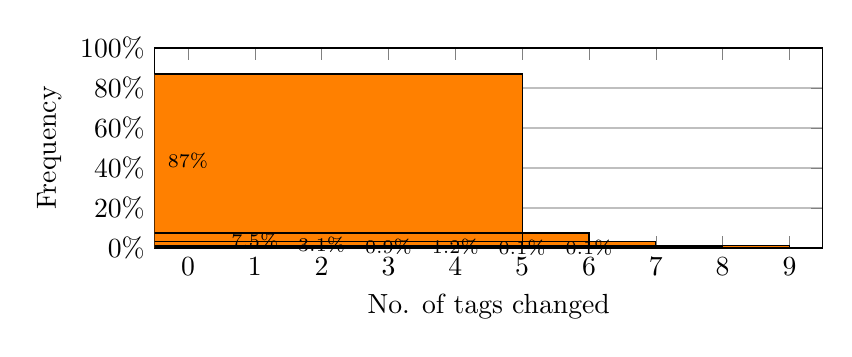
\begin{tikzpicture}
\begin{axis}[
	ybar stacked,
	width=0.7\columnwidth,
	height=1in,
	scale only axis,
	xtick=data,
	xlabel={No. of tags changed},
	ylabel={Frequency},
	point meta={y*100},
	nodes near coords={\scriptsize\pgfmathprintnumber\pgfplotspointmeta\%},
	yticklabel={\pgfmathparse{\tick*100}\pgfmathprintnumber{\pgfmathresult}\%},
	try min ticks={4},
%	x label style={yshift=10pt},
	y label style={},
	ymin=0.0,ymax=1.0,
	xmin=-0.5, xmax=9.5,
    bar width=10,
    log basis y=10,
    ymajorgrids
]

\addplot [fill=orange]
	coordinates {(0, .87)	(1, .075)	(2, .031)	(3, .009)	(4, .012)	(5, .001)	(6, .001)	(7, 0)	(8, 0)	(9, 0)};

\end{axis}
\end{tikzpicture}
\caption{Distribution of number of tags changed each time the chunker is run with one additional word.}
\end{figure}

The use of conditional random fields complicates the analysis somewhat because adding a word can affect the tags of words already processed, which causes the tree structure to change. In this case, we recompute all nodes in the tree corresponding to words with changed tags, paying the recomputation penalty. Other models such as Hidden Markov Models also have this property.


\begin{figure*}[!t]
  \centering
  \setlength\extrarowheight{0pt}
  \fbox{
  \begin{tabularx}{0.95\textwidth}{@{}c X@{}}
  \multirow{6}{0.95\columnwidth}{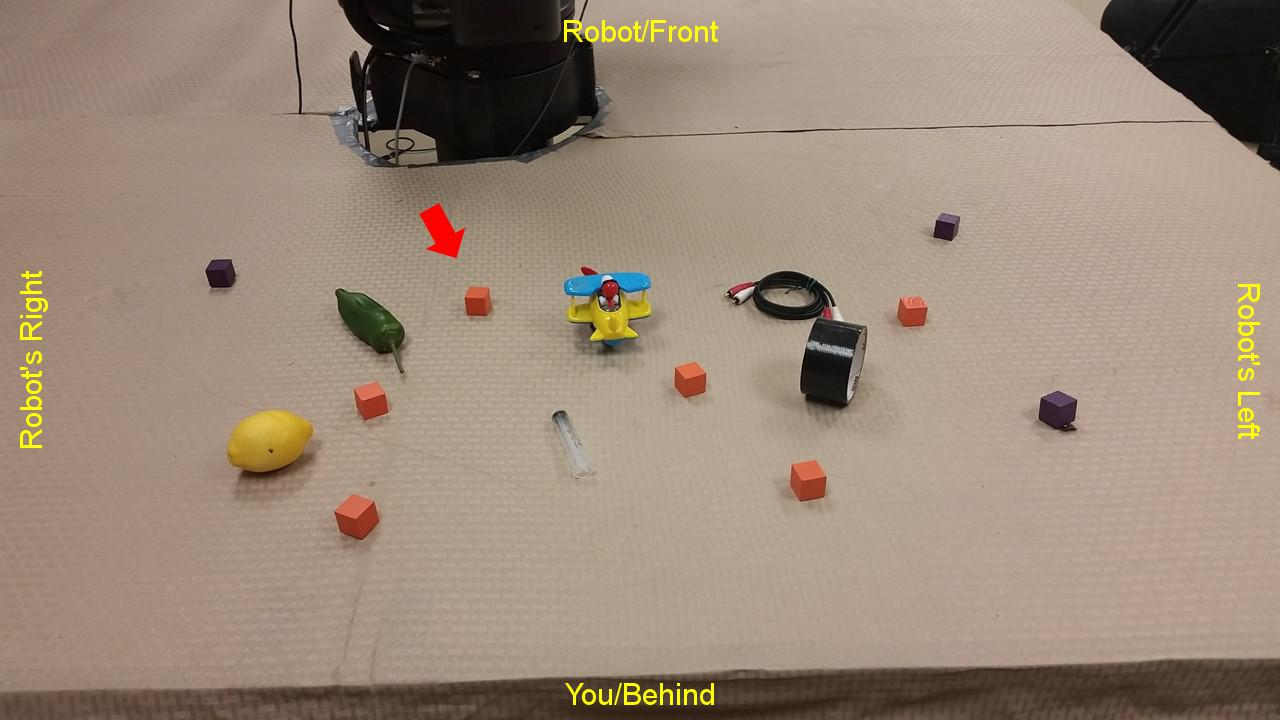
\includegraphics[width=0.95\columnwidth]{ref_expr_examples_pic}}
    & Examples of responses from AMT workers: \\
	& ``I want the orange cube in front of you, between the chili and the toy.'' \\
	& ``hand me the orange cube that is in between jalape\~{n}o and airplane'' \\
	& ``Directly in front of you next to the green pepper and airplane.'' \\
	& ``Take the orange block between the toy airplane and green chili pepper'' \\
	& ``bring the orange cube between the pepper and the plane.'' \\ 
   	\end{tabularx}
    }
	\caption{Example picture provided to AMT workers to elicit referring expressions and sample responses.}
	\label{fig:ref_expr_examples_pic}
\end{figure*}

We choose to use Conditional Random Fields in part because we can explicitly set the look-ahead limit, and so pick a tradeoff between tagging accuracy and potential worst-case performance. For our algorithm, we arbitrarily set it to 5.

The worst-case runtime scales linearly with the look-ahead limit. To characterize the typical performance penalty caused by our choice of look-ahead parameter, we gathered statistics on the likelihood of this happening in our training set.

We found that, in our test set, each time a word is added an average of 0.23 earlier tags are changed. The observed distribution is presented in Figure~\ref{fig:crf_retagging_hist}. The $95^\text{th}$ percentile case is still within the same order of magnitude as the case without any changes.


\section{Evaluation} 

We collected a corpus of human-generated data using Human Intelligence Tasks (HITs) on the Amazon Mechanical Turk (AMT) platform and hand-generated scenes. We additionally use AMT to have humans evaluate our test set to obtain a baseline. We trained the language model and spatial-prepositional model on a training set of 11 scenes, each with an average of 14 objects, for a total of 417 input sentences. We trained the chunker on hand-annotated parses of these input sentences.

 \subsection{Data Collection}
A set of HITs were created to elicit referring expressions. A total of 19 scenes were constructed, each with a set of about 12 to 15 objects scattered on a table and at least 6 identical orange cubes. For each orange cube in each scene, 9 different workers were told to ask a robot across the table for the indicated orange cube. Figure~\ref{fig:ref_expr_examples_pic} provides an example of such a labeled scene.

We provide the following instructions:

\begin{framed}
You are standing across the table from a robot. Write down what you would say to the robot if you wanted the indicated orange cube on the table.
\begin{itemize}[topsep=0pt,itemsep=-1ex,partopsep=1ex,parsep=1ex,leftmargin=1em]
\item Use phrases like "between", "near", "left of", "right of", "in front of" and "behind".
\item Use front/behind/left/right from the robot's perspective, as labeled in the image. 
\item All orange cubes look the same.
\item You must ask for the item indicated by the red arrow
\item The instruction must be a single sentence.
\end{itemize}
\end{framed}

For each referring expression in the test set, we get three separate human raters to identify the target and provide feedback on the ease of understanding of the referring expression. Figure~\ref{fig:ref_expr_eval_pic} shows an example scene. Refer to Figure~\ref{fig:results} for how often humans correctly identify the target, and Figure~\ref{fig:interrater} for interrater agreement.  

\begin{figure}[!h]
  \centering
    \fbox{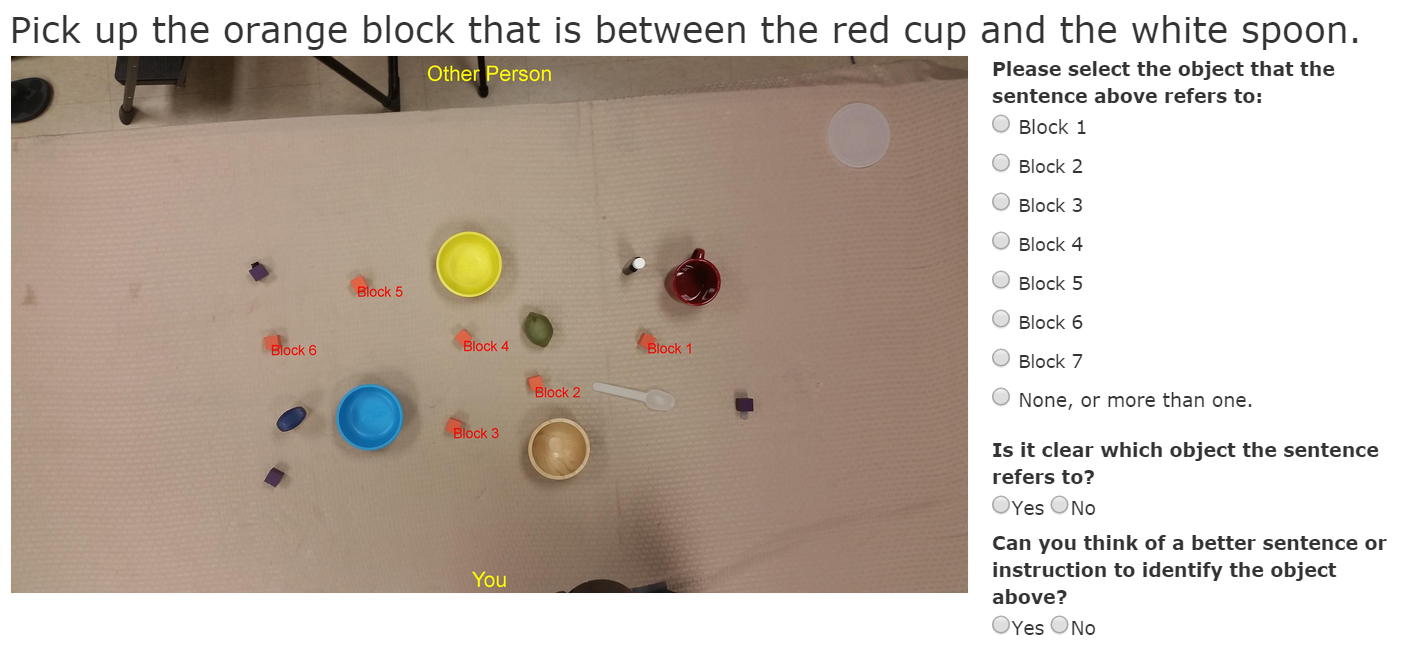
\includegraphics[width=0.95\columnwidth]{ref_expr_eval_pic}}
  \caption{Example picture provided to AMT workers to evaluate referring expressions.}
  \label{fig:ref_expr_eval_pic}
\end{figure}


\begin{figure*}[!b]
  \centering
  \begin{tabular}{| r r | c | c | c || c c |} \hline
     & & \multicolumn{5}{c|}{Rate of correct identification, Test (\%)} \\
     & & \multicolumn{3}{c||}{Baselines} & \multicolumn{2}{c|}{Results} \\
     \multicolumn{2}{|c|}{Preposition}
			                      &   Human & Unigram & Random &  Top-1 & Top-3 \\\hline
26.8\% & \textit{between}       & 88.2  & 14.3  & 7.1   & 71.6  & 94.1 \\
21.3\% & \textit{near}          & 82.5  & 17.2  & 7.3   & 7.9   & 51.1 \\
14.2\% & \textit{behind}        & 76.9  & 15.7  & 6.9   & 25.9  & 75.9 \\
11.0\% & \textit{in front of}   & 69.9  & 17.9  & 7.5   & 21.4  & 64.3 \\
9.4\% & \textit{left of}        & 89.8  & 16.1  & 7.3   & 25.0  & 83.3 \\
5.8\% & \textit{right of}       & 58.0  & 15.4  & 7.3   & 32.5  & 55.2 \\\hline\hline
    \multicolumn{2}{|r|}{Total} & 79.0  & 16.1  & 7.2   & 32.8  & 63.5 \\\hline
  \end{tabular}
  \caption{Performance on test set.}
  \label{fig:results}
\end{figure*}

\subsection{Results}

After training our model on the training set, we tested it using a test set of 10 scenes, each with an average of 14 objects, for a total of 381 input sentences. The result of running the parser on complete referring expressions is in Figure~\ref{fig:results}.

Figure~\ref{fig:results} shows the correctness rate of our algorithm and of three baselines for comparison. The percentage next to each preposition is the fraction of sentences in the test set that contain this preposition, and so will not add up to 100\%. The baselines are:
\begin{enumerate}[topsep=0pt,itemsep=-1ex,partopsep=1ex,parsep=1ex]
	\item The \emph{Human} baseline, which was established by having humans select the object best identified by the referring expression, and scoring them against our corpus.
	\item The \emph{Unigram} baseline, which is the expectation of selecting the correct object using a simple unigram object model across the entire input sentence.
	\item The \emph{Random} baseline, which is the expectation of selecting the correct object by selecting one object uniformly at random.
\end{enumerate}

The \emph{Results} column lists the rate of correct identification using the entire sentence as input, the \emph{Top-1} column lists the rate at which the correct object is rated the most likely by the algorithm, and the \emph{Top-3} column lists the rate at which the correct object is in the top 3 items.

For evaluation, the rate of correct identification is the number of trials in which the algorithm assigns a higher probability to the correct item than to any other item. Should there be a tie, the rate is divided by the number of items of equal probability.

The percentage on the left of each preposition is the fraction of the test set that contains that preposition.

To evaluate incremental performance, we report performance on the test set as a fraction of each sentence provided to the algorithm. Figure~\ref{fig:results_inc} reports the evaluation of the test set when our algorithm is run on it word-by-word. Note that, due to the variation in lengths of sentences, the charts are drawn by interpolating fraction of each sentence into bins from 0 to 1.

\begin{figure}[h]
  \centering
  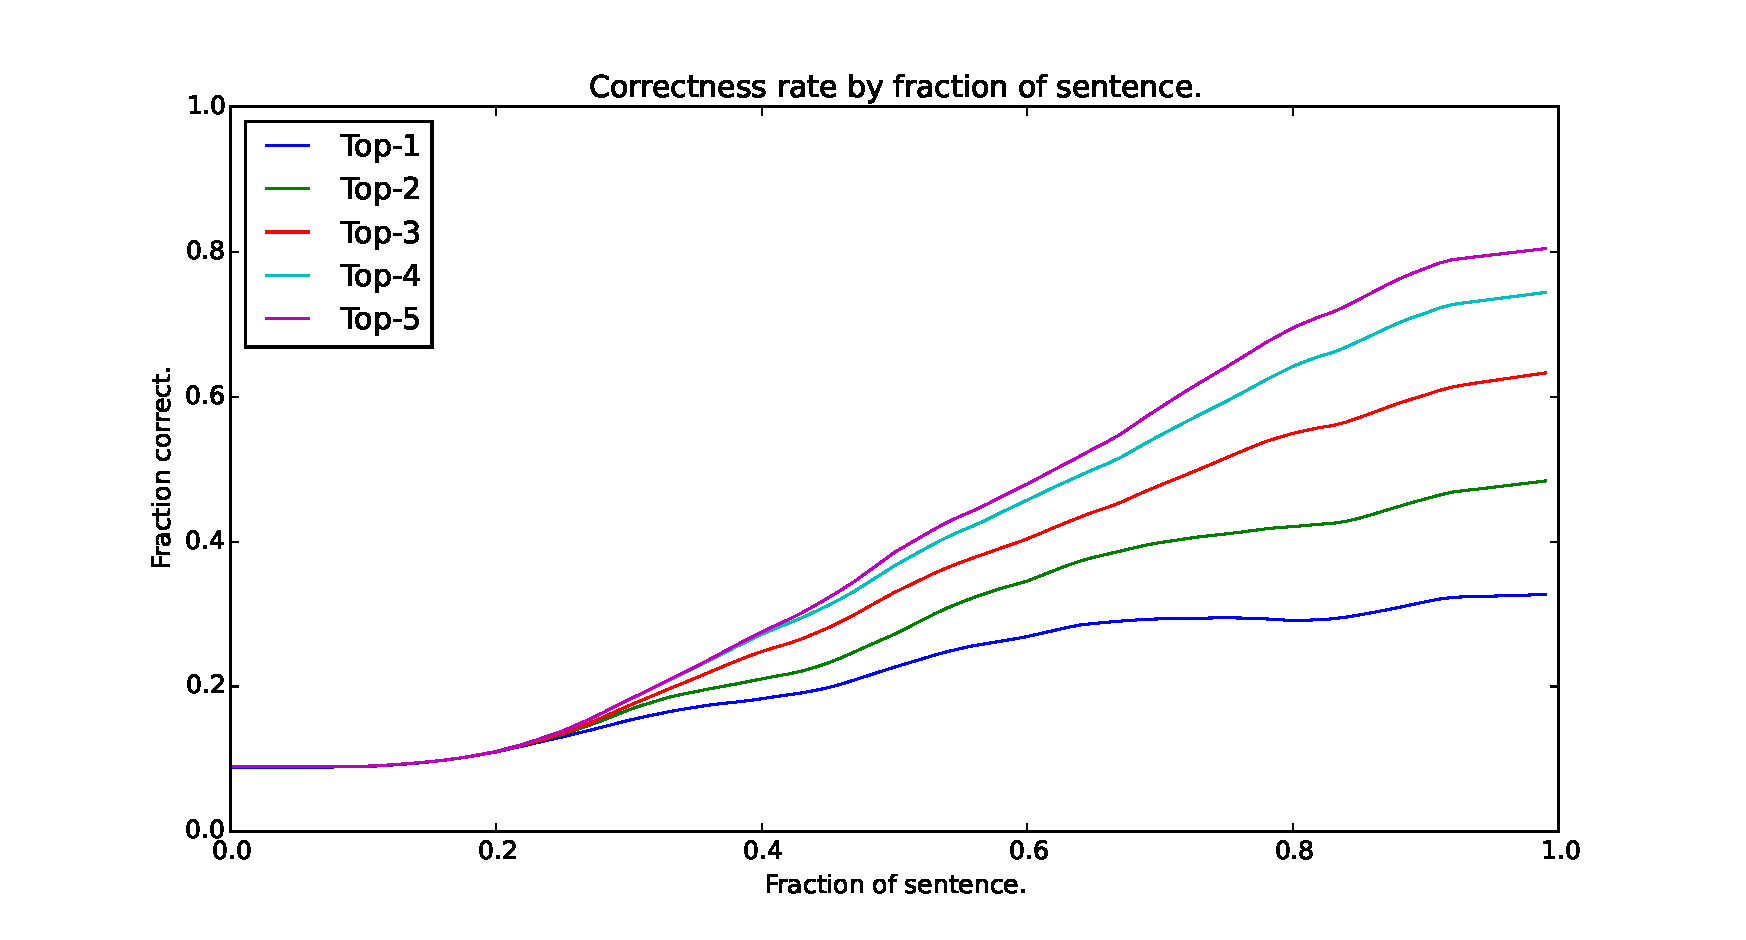
\includegraphics[width=\columnwidth]{eval/cdf_by_fraction}
  \caption{Performance on test set.}
  \label{fig:results_inc}
\end{figure}

Five separate lines are drawn to show the distribution of the rank of the correct option. Each Top-$k$ line includes an example if the target object has at least as much probability as the $k^\text{th}$-highest probability in the distribution. Should there be a tie, the rate is divided by the number of items of equal probability.

\subsection{Failure Analysis}
After testing was complete, we examined individual cases in the test set to characterize failures. 

\subsubsection{Spatial Model of `near'}

We observe that the rate of correct identification of our model is particularly low in comparison to that of humans when dealing with the preposition `near'. For each phrase ``[Figure] near [Landmark]'' in the training and test sets, we plot the location of the ``Landmark'' object in comparison to the target ``Figure'' object in in the training and test sets in Figure~\ref{fig:near_comp}. It is clear that this simple model does not fully capture the nuances of the use of `near'.

\begin{figure}[h!tb]
  \centering
    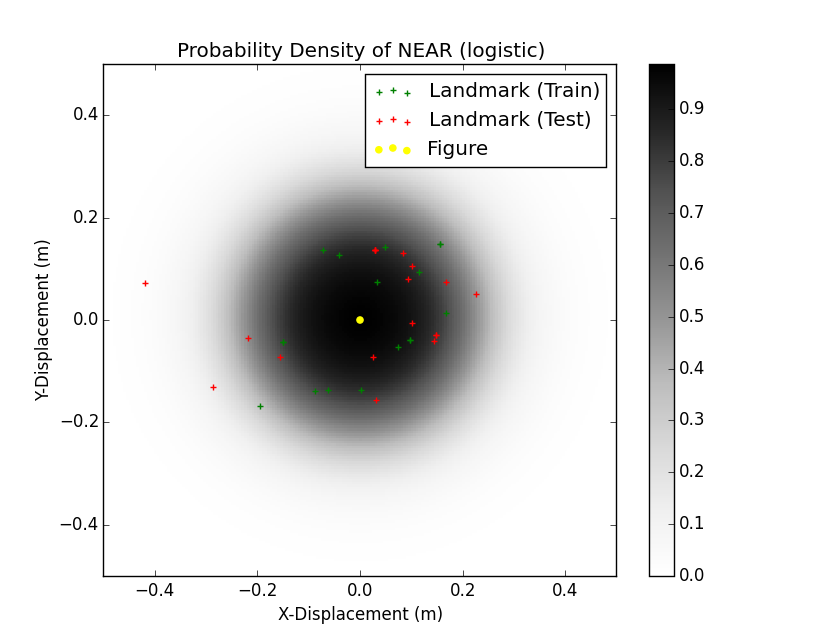
\includegraphics[width=1.1\columnwidth]{near_train_test_comp}
  \caption{Relative position of ``[Figure] near [Landmark]'' in the training and the test sets, with the probability density of the model as background.}
  \label{fig:near_comp}
\end{figure}

Perhaps this model could be extended to include the relative positions of other objects, or to reflect the local geometry of the scene. We suspect that a major source of error is the difference in perspective of the robot and the human. The human perspective is in front of the table and so is subject to foreshortening, while the robot's perspective does not.

\subsubsection{Dealing with Imprecise and Incorrect Data}

Another major source of error is the presence of imprecise or incorrect data in our training and test set. An imprecise referring expression is one that does not uniquely identify a target object, and an incorrect referring expression is one that does not identify the correct object. Here we estimate how much of our error is due to imprecise and incorrect referring expressions by evaluating our algorithm on referring expressions with $r$ humans correctly identifying the target object.

Figure~\ref{fig:interrater} shows the outcome of this when we restrict the test set to referring expressions that have been correctly identified by an increasing number of humans. The first column is the control (using all data), the second includes only referring expressions correctly solved by at least one human, then at least two humans, and finally only those by all three humans.

\begin{figure}[h!tb]
  \centering
  \begin{tabular}{|r|m{1.2cm}m{1.2cm}m{1.2cm}m{1.2cm}|}\hline
  & \multicolumn{4}{c|}{Rate of correct identification, Test (\%)} \\
  $r$ & $\geq 0$ & $\geq 1$ & $\geq 2$ & $=3$ \\\hline
  Top-1 & 32.8 & 33.7 & 34.2 & 36.9 \\
  Top-3 & 63.5 & 65.3 & 65.9 & 69.6 \\\hline
  (\%) & 100 & 93.1 & 84.5 & 59.3 \\\hline
  \end{tabular}
  \caption{Correctness rate for different number of correct raters, with size of data.}
  \label{fig:interrater}
\end{figure}

From this we see that genuine confusion accounts for between 4-6 percentage points of the total error, which is substantial.

\section{Related Work}

Prepositional phrases have not been subject to as much computational analysis and study as noun- and verb-phrases. However, there are still a number of papers related to the topic. 

There is an existing family of related work by \citet{tellex2011understanding}, \citet{UW_RSE_ICML2012}, and \citet{artzi2013weakly}, all of whom present modern models to process referring expressions. These models all operate on entire input sentences and are designed to parse general instructions and commands instead of only prepositional phrases. 
\citet{tellex2011understanding} present the $G^3$ framework. We use several key ideas from this paper: in particular we implicitly assume the binary correspondence variable that their model maximizes. Our algorithm is inspired in part by the algorithm they present.
\citet{UW_RSE_ICML2012} present a state-of-the-art process to learn models for a semantic parser and word-classifier alignment. Our approach is substantially different from Matuszek~et.~al. since we do not separate perceptual features from the language model of each object. Also, in the learning phase of their algorithm, they calculate the marginal probability of a particular grounding and a particular word by performing a beam search over all possible parses. We assume instead that each node in the parse is independent of its sibling nodes, which allows us to use dynamic programming to incrementally build the distribution.
\citet{artzi2013weakly} train Combinatory Categorial Grammars (CCG) with ambiguous validation functions to parse instructions, including spatial relations. While this approach is more flexible and likely performs better on entirely novel sentences, we deliberately choose a simpler model that lends itself to a dynamic programming approach.

\citet{fang2015embodied} present a model to collaboratively generate a referring expression, incorporating feedback from the human subject to generate additional terms. The paper focuses on the generation of referring expressions and the use of gestural feedback, and so is of limited use in the context of this paper.

In addition to these, we rely on previous work about prepositional phrases:

\citet{collins95} present a model for disambiguating prepositional phrase attachments. They deal with Noun-Phrases and Verb-Phrases, but their statistical technique may be useful. This concept is also explored by \citet{ratna98}, and \citet{brill94}, each of whom suggest alternative models. Additionally, \citet{merlo97} explore disambiguating multiple prepositional phrases, rather than a single phrase between multiple targets, both of which are relevant to future work. However, our current model uses sentences focused around a single noun phrase, unlike the general English corpus used in this paper. Additionally, the incremental nature of our parsing requires an alternative framework, and as such not all techniques suggested in these papers can be used.

Another issue we face is the challenge of identifying objects and mapping them to probability distributions via language model. To deal with this, \citet{barbu13} present a model for mapping language to object models in video data and \citet{UW_RSE_ICML2012} describe an approach to the problem of simultaneously observing and extracting representations of a perceived world. These approaches can be adapted to help design features, choose objects, and select language models for prepositional phrase training, rather than using pre-defined objects and locations as we currently do, similar to the work of \citet{tellex2011understanding} which presents a method to dynamically generate a probabilistic model of a natural language input and perform inferences relating to semantic meaning. This is similar to the work we will preform in semantic parsing, though we will do so incrementally rather than with an entire sentence and thus our work will need to modify these models.

There are still a number of improvements to be made to our machine learning techniques. \citet{rudzicz03} give us a framework for parsing and understanding prepositional phrases. Similarly, \citet{liang2013learning} describe a method to create a semantic parser using question-answer pairs as data, rather than requiring annotated sentences, solving the same issue we approach of transforming natural language into semantic meaning. However, while these may be useful for generating a semantic model over entire sentences our technique will be different as we are currently only working with noun phrases, and apply additional information from the spatial model. 

\section{Conclusion}
In this paper we have presented an incremental referring expression parser that can process prepositional phrases. The incremental nature of the parser is the key contribution: state-of-the-art parsers all operate on complete referring expressions. 

The primary future task is to integrate this with the social feedback framework on Baxter in the H2R lab and conduct user studies to investigate if this provides a measurable improvement to user interaction. Other future work includes developing a model of the preposition `near' that better matches human sensibilities. This may even extend to learning the spatial shift between humans and our system and adjusting spatial models to account for that.

From an algorithmic development perspective, a natural extension of this algorithm is to replace the chunking and semantic tree construction with a chart parser. The chart parser will provide an incremental model of parsing that our spatial model can be directly integrated into. This may even allow the spatial model to inform the parsing, such as by increasing the probability of parses that correspond to narrower distributions. The increased power of the model would be the greater computational overhead: further analysis and experimentation is required to see if this is suitable for use in interactive scenarios.

\section{Acknowledgments}
This thesis project is the culmination of work done from Fall 2014 to present. Some work was previously completed in collaboration with undergraduate student Zachary Loery.

This project was completed in the H2R laboratory in the Brown computer science department, with Prof. Stefanie Tellex as advisor.


\printbibliography

\end{document}

